% Kaleidoscope mirror cutting template — 100 mm prototype.
% Trapezoid: parallel edges 25.40 / 50.80 mm, height 100.268 mm, legs 101.070 mm.
% Everything is drawn 1:1. Do not scale this file when printing.
\documentclass[letterpaper,11pt]{article}
\usepackage[letterpaper,top=11mm,bottom=10mm,left=13mm,right=13mm]{geometry}
\usepackage{tikz}
\usepackage{xcolor}
\usetikzlibrary{arrows.meta}
\pagestyle{empty}
\setlength{\parindent}{0pt}
\definecolor{reg}{gray}{0.45}

% corner registration mark: prick through the centre with a pin
\newcommand{\cmark}[2]{%
  \draw[reg,line width=0.18mm] ({#1},{#2}) circle (1.4mm);
  \draw[reg,line width=0.18mm] ({#1-2.8},{#2}) -- ({#1+2.8},{#2});
  \draw[reg,line width=0.18mm] ({#1},{#2-2.8}) -- ({#1},{#2+2.8});
}

\newcommand{\Hgt}{100.268}

\begin{document}

\begin{center}
  {\large\bfseries Kaleidoscope mirror cutting template}\\[0.8mm]
  {\small 100\,mm prototype \quad\textperiodcentered\quad three identical mirrors
   \quad\textperiodcentered\quad drawn 1:1}
\end{center}

\vspace{1mm}
\fbox{\parbox{\dimexpr\linewidth-2\fboxsep-2\fboxrule\relax}{\small
\textbf{Print at 100\%.} In the print dialog choose \emph{Actual size} or \emph{100\%} —
not \emph{Fit to page}, not \emph{Shrink oversized pages}. Then check \emph{both} rulers
below with a real ruler before you cut anything. If they are off, so is every dimension
on this page.}}

\vspace{3mm}

% ── horizontal scale check ────────────────────────────────────────────────
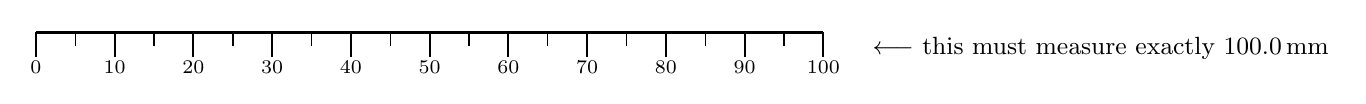
\begin{tikzpicture}[x=1mm,y=1mm]
  \draw[line width=0.35mm] (0,0) -- (100,0);
  \foreach \i in {0,10,...,100} {
    \draw[line width=0.25mm] (\i,0) -- (\i,-3.2);
    \node[below,font=\scriptsize,inner sep=1pt] at (\i,-3.2) {\i};
  }
  \foreach \i in {5,15,...,95} { \draw[line width=0.18mm] (\i,0) -- (\i,-1.8); }
  \node[right,font=\small] at (105,-2) {$\longleftarrow$ this must measure exactly 100.0\,mm};
\end{tikzpicture}

\vspace{5mm}

% ── the parts, with a vertical scale check alongside ──────────────────────
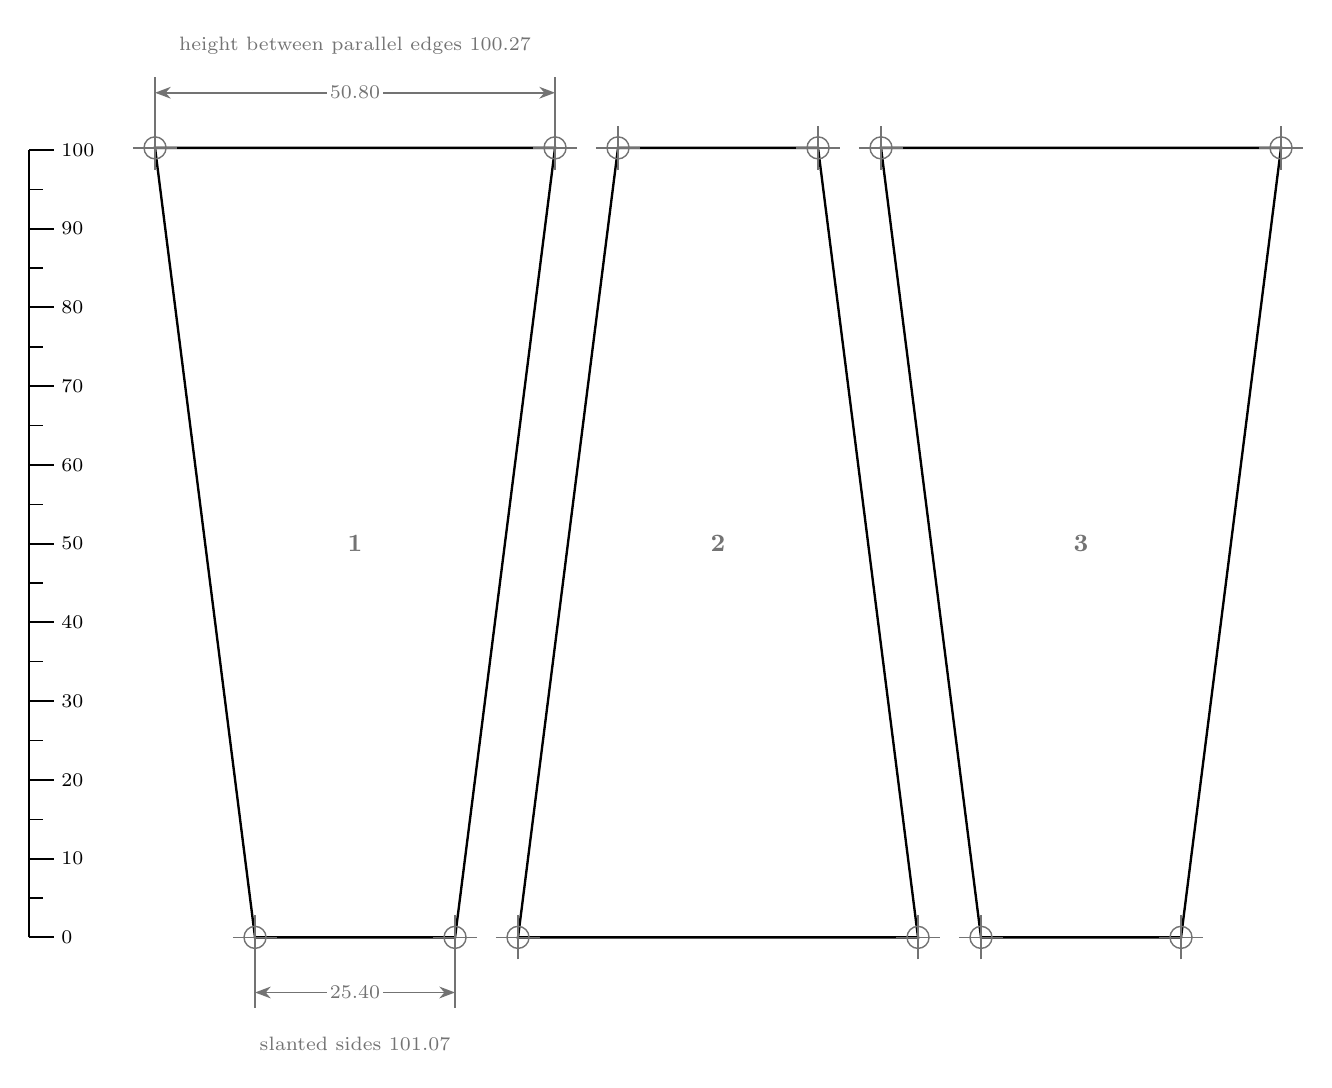
\begin{tikzpicture}[x=1mm,y=1mm,line width=0.30mm]

  % vertical 100 mm ruler
  \draw[line width=0.35mm] (0,0) -- (0,100);
  \foreach \i in {0,10,...,100} {
    \draw[line width=0.25mm] (0,\i) -- (3.2,\i);
    \node[right,font=\scriptsize,inner sep=1pt] at (3.6,\i) {\i};
  }
  \foreach \i in {5,15,...,95} { \draw[line width=0.18mm] (0,\i) -- (1.8,\i); }

  % ── mirror 1 : narrow edge at the bottom ──
  \draw (28.7,0) -- (54.1,0) -- (66.8,\Hgt) -- (16.0,\Hgt) -- cycle;
  \cmark{28.7}{0}\cmark{54.1}{0}\cmark{66.8}{\Hgt}\cmark{16.0}{\Hgt}
  \node[font=\small\bfseries,reg] at (41.4,50) {1};

  % ── mirror 2 : flipped, wide edge at the bottom ──
  \draw (62.1,0) -- (112.9,0) -- (100.2,\Hgt) -- (74.8,\Hgt) -- cycle;
  \cmark{62.1}{0}\cmark{112.9}{0}\cmark{100.2}{\Hgt}\cmark{74.8}{\Hgt}
  \node[font=\small\bfseries,reg] at (87.5,50) {2};

  % ── mirror 3 : narrow edge at the bottom ──
  \draw (120.9,0) -- (146.3,0) -- (159.0,\Hgt) -- (108.2,\Hgt) -- cycle;
  \cmark{120.9}{0}\cmark{146.3}{0}\cmark{159.0}{\Hgt}\cmark{108.2}{\Hgt}
  \node[font=\small\bfseries,reg] at (133.6,50) {3};

  % dimensions, shown once on mirror 1
  \draw[reg,line width=0.15mm] (28.7,0) -- (28.7,-9);
  \draw[reg,line width=0.15mm] (54.1,0) -- (54.1,-9);
  \draw[reg,line width=0.2mm,{Stealth[length=2mm]}-{Stealth[length=2mm]}]
        (28.7,-7) -- (54.1,-7) node[midway,fill=white,inner sep=1pt,font=\scriptsize]{25.40};

  \draw[reg,line width=0.15mm] (16.0,\Hgt) -- (16.0,\Hgt+9);
  \draw[reg,line width=0.15mm] (66.8,\Hgt) -- (66.8,\Hgt+9);
  \draw[reg,line width=0.2mm,{Stealth[length=2mm]}-{Stealth[length=2mm]}]
        (16.0,\Hgt+7) -- (66.8,\Hgt+7) node[midway,fill=white,inner sep=1pt,font=\scriptsize]{50.80};

  \node[reg,font=\scriptsize] at (41.4,-13.5) {slanted sides 101.07};
  \node[reg,font=\scriptsize] at (41.4,\Hgt+13) {height between parallel edges 100.27};

\end{tikzpicture}

\vspace{4mm}
\hrule
\vspace{2mm}

{\small
\textbf{How to use it.} Leave the protective film on the mirror. Tape this sheet down
over it, prick through the centre of all twelve circled marks with a pin or a scribe,
lift the paper off, then join the pricks with your straightedge and score along those
lines. Marking through the paper is more accurate than trying to cut through it — a
knife shreds paper and then wanders.

\smallskip

\textbf{Cut on the line.} These outlines are the finished size and carry no allowance.
A scored-and-snapped edge removes essentially nothing, so cut right on the marks. If you
ever laser-cut these, offset the toolpath \emph{outward} by half the kerf, or the mirrors
come out undersized and leave a gap at every corner.

\smallskip

\textbf{Only two edges matter.} The slanted 101.07\,mm sides are the ones that butt against
the neighbouring mirrors — they must be straight, and the reflective coating must run right
to the edge. The 25.40 and 50.80\,mm ends are hidden under the end caps and can be rough.

\smallskip

\textbf{There is no left or right.} Each trapezoid is symmetric, so all three pieces are
interchangeable and either face can end up outward. The handedness in this design lives in
how the three are \emph{assembled}, not in how they are cut. Mirror 2 is drawn flipped only
to nest the three efficiently on the tile.
}

\end{document}
